

\pagebreak 
%\section{Evaluation of Automatic Stabilizers}
\section{Stabilization in the Presence of Unemployment Risk}
Incomplete markets for households along with matching frictions generates countercyclical precautionary savings as households attempts to self-insure against unemployment risk over the cycle. This section takes a closer look at how unemployment benefits - which acts as insurance against unemployment shocks - affects the economy over the business cycle. This includes both effects on aggregates in the general equilibrium and distributional and welfare effects.    

Note that unemployment risk essentially works by fluctuation households between a good state (employment) and a bad state (unemployment). When unemployment benefits are reduced the bad state becomes even worse when compared to the good state. This is comparable to the zero-income shock in \citet{carroll1997buffer}, which he argues is a significant driver of savings for precautionary  reasons. 



%I primarily focus on the stabilizing effects of unemployment benefits over the business cycle. I do this for several reasons. Unemployment benefits interact directly with the demand side through the household sector, and hence has the possibility to be a strong stabilizer since output is demand driven in the short run in NK models. Furthermore, in models with heterogeneous agents unemployment benefits affect precautionary savings motives through both income levels and labor market channels (job-finding rates). Lastly, since this particular stabilizer is associated with the redistribution of income it can be a significant source of distributional effects over the cycle.  


\subsubsection{A new Steady State}
I conduct the following experiment:
A permanent drop in the unemployment benefit rate is phased in over 100 quarters. After 300 quarters the model is assumed to have converged to a new, counterfactual steady-state which mimics the basic properties of the original steady-state, with the exception of having a lower unemployment benefit rate. To evaluate the stabilizing properties of unemployment benefits I then subject each of the steady-states to a negative TFP shock similar to the one described earlier. For unemployment benefits shock I let lump-sum transfers adjust such that the government debt-to-GDP ratio is the same as in the original steady-state (160\%).

\newcommand{\dBenefitRate}{50\%}

Figure \ref{fig:Lower_b_Transitional} in the appendix shows the responses to the permanent benefits shock. The shock lowers the benefit level by \dBenefitRate, with a phase in period corresponding to a auto-regressive parameter of 0.95.\footnote{\citet{mckay2016role} considers a  80\% reduction in  unemployment and poverty benefits.} The new steady-state is of course in itself of interest, as it touches upon the literature concerning the relation between unemployment benefits and employment, production and wages. However, in that regard the model misses the moral hazard channel of unemployment benefits affecting the extensive labor market margin, which is a major channel in this discussion. Note also that had the model included Nash-bargaining over wages, the level of unemployment benefits would have a direct effect on the bargained wage through its interpretation as the outside option. This channel is omitted in the model. \\

The drop in unemployment benefits implies a permanent drop in consumption due to lower income and precautionary savings. The drop in demand induces firm to investment less and hire less workers, so the stock of capital drops and the unemployment rate increases. This further increases the drop in consumption. The permanent increase in unemployment implies a permanently less tight labor market for firms, and hence lower wages. Since wages adjust endogenous to the drop in unemployment benefits the replacement ratio $b/w$ is in itself endogenous, and hence can be either higher or lower than the 25\% implied by the calibration and the drop in benefits of \dBenefitRate. However, according to Figure \ref{fig:Lower_b_Transitional} wages drop only marginally by 0.03\%, so the replacement rate drop by roughly \dBenefitRate - a sizeable amount.   
Relative to the old steady-state the aggregate stock of assets increase by 2.5\% for precautionary reasons. Figure \ref{fig:lower_b_dA} shows that this increase is driven entirely by employed households. The income of these households are affected only marginally in the new steady-state, but and they can thus afford to increase their insurance against unemployment through assets. This channel is strongest for households in the bottom of the wealth distribution since these are particularly poor insured to begin with. Unemployed households respond to the drop in benefits by drawing on their buffer of assets to increase consumption such that assets drop. Unemployed households at the bottom of the wealth distribution has a smaller decrease in assets due to borrowing constraints. The fact that constrained households cannot insure to the extent of their wish potentially imply large welfare losses. 

\begin{figure}[H]
\makebox[\linewidth][c]{%
\centering
  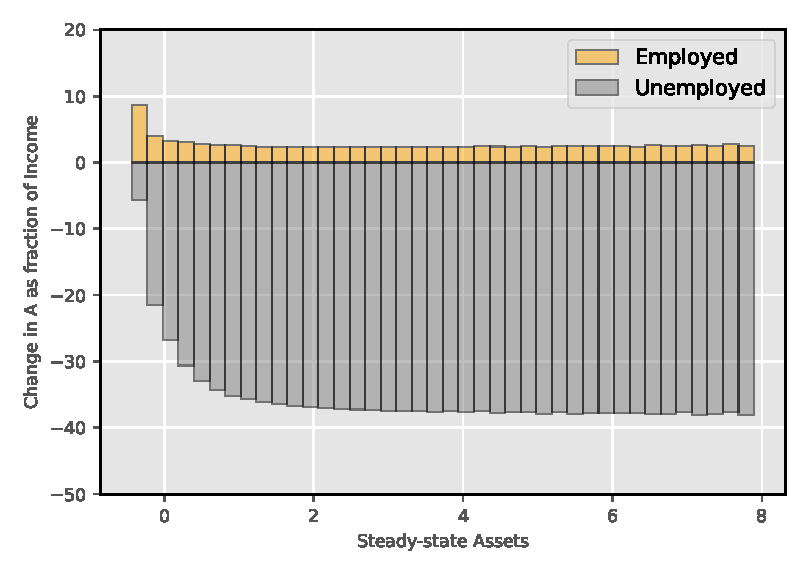
\includegraphics[width=.6\linewidth]{mainmatter/plots/Lower_b_main/dA.pdf} 
}
\caption[Caption for LOF]{Change in Assets by initial steady-state assets.}
\label{fig:lower_b_dA}
 % {\scriptsize  Impulse responses to a negative productivity shock of 1\% with persistence 0.94 (half-life: 5 quarters). }
\end{figure}

Figure \ref{fig:Lower_b_Transitional} shows the estimated transitional dynamics using both linear and non-linear methods. Due to the size of the shock non-linearities matter, and I hence use the non-linear method to iterate to the new steady state. 


\subsubsection{Unemployment Benefits as a Stabilizer}
Having numerically obtained the new steady state with a lower level of unemployment benefits, I now investigate the stabilizing properties of these benefits. Figure \ref{fig:lower_b_main} compares negativity productivity shock (1\% with persistence 0.8) in the baseline model and the model with lower unemployment benefits.
The on-impact drop in consumption is greatly affected by the amount if unemployment insurance (-2\% vs -2.5\%), though the afterwards persistence is roughly the same. This drop in demand leads to larger drops in employment and output, though investment seems to be unaffected. The reduction of labor demand diminishes job-finding opportunities, and the labor market becomes less tight from the point of view of firms. This leads to a further drop in wages and hours worked. The drop in employment and output implies a slight drop in marginal costs and hence inflation. In turn, the central bank raises the interest rate less. 

%Somewhat surprisingly given the size of the shock to benefits, the remaining business cycle variables are relatively unaffected, and the majority are actually stabilized by the lower level of benefits. This derives primarily from a general equilibrium effect working through the governments budget. As the economy deteriorates following the shock, unemployment rises and hence public expenses associated with unemployment benefits increases. This is primarily financed by issuing debt, but also by cutting government spending. In the model with lower benefits the expenditure side of the government budget suffers less and public consumption is cut by less. Since this is in itself a component of aggregate demand, there is a slight drop in volatility. The reduced volatility in employment, job finding rates etc. is, however not sufficient to counter the drop in consumption occurring through the lower value of unemployment. 



%The immediate conclusion is that the level of unemployment benefits and hence the replacement ratio does not affect the persistence of shocks, and does little towards the size and propagation of the negative investment shock. While the quantitative effects are small, the qualitative effects reflect that unemployment benefits does serve a purpose as a stabilizer: It lessens the drop in consumption, output and employment.  

\begin{figure}[H]
\makebox[\linewidth][c]{%
\centering
  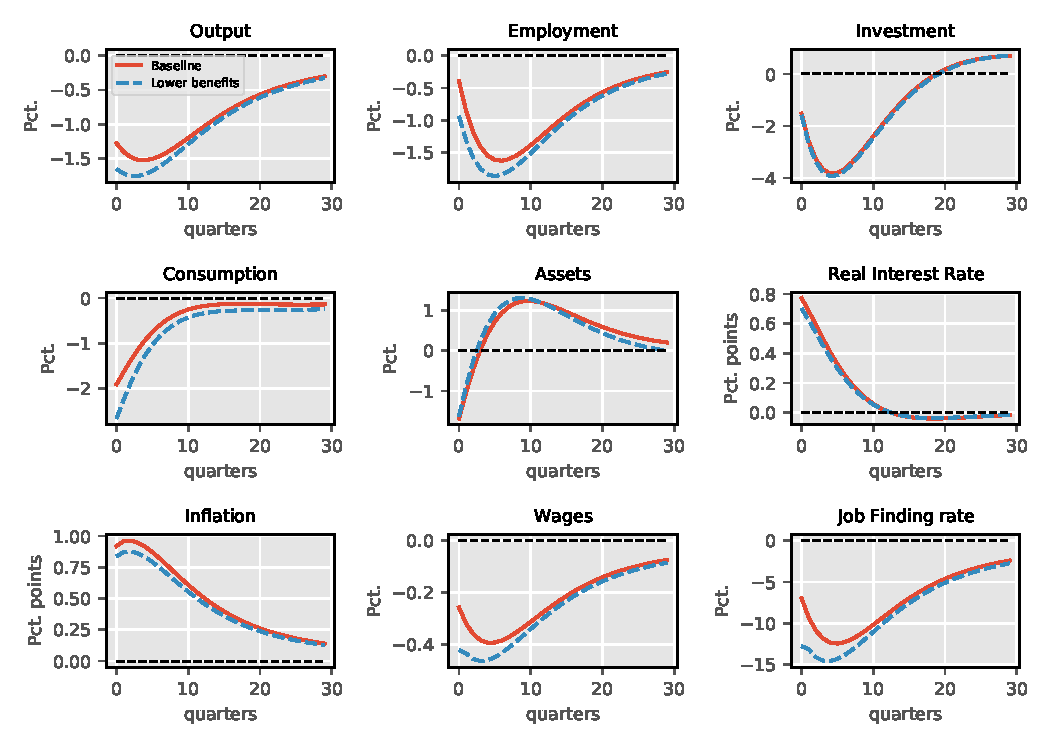
\includegraphics[width=.8\linewidth]{mainmatter/plots/Lower_b_main/main_result_comparison_G.pdf} 
}
\caption[Caption for LOF]{Impulses to a negative TFP shock with standard and low unemployment benefits.}
\label{fig:lower_b_main}
 % {\scriptsize  Impulse responses to a negative productivity shock of 1\% with persistence 0.94 (half-life: 5 quarters). }
\end{figure}

%Unemployment benefits directly affect the model into places: The income process of household and the government's budget constraint. Figure \ref{fig:lower_b_C_decomp} 


Figure \ref{fig:lower_b_C_decomp_G} decomposes the aggregate response of consumption. The figure reveals that the level of unemployment benefits is important for the response of consumption to changes in employment and job-finding opportunities. The drop in job-finding rates has a strong, immediate negative effect on consumption (roughly double the effect on impact) under lower benefits due to a stronger precautionary motive: For employed households lower job-finding rates imply that if they drop into unemployment exogenously their odds of bouncing back into employment diminishes. Hence they buffer up on assets by cutting consumption to ensure against this increased risk. For unemployed households future employment prospects drop, and they increase savings to accommodate a longer unemployment spell. A more severe drop in employment in the general equilibrium generates a more persistent drop in consumption since unemployed households on average has lower consumption.\footnote{At a benefit rate of 51\% (the baseline model) unemployed households has on average 86\% the consumption of employed households. After the cut in benefits this figure drop to 80\%.} Wages decline more in the general equilibrium of the modified model and this leads to a larger consumption drop. The response of consumption to changes the interest is roughly the same. 

Essentially, the drop in unemployment benefits have not dramatically large effects in the general equilibrium because households manage to self-insure against unemployment risk. 

\begin{figure}[H]
\makebox[\linewidth][c]{%
\centering
  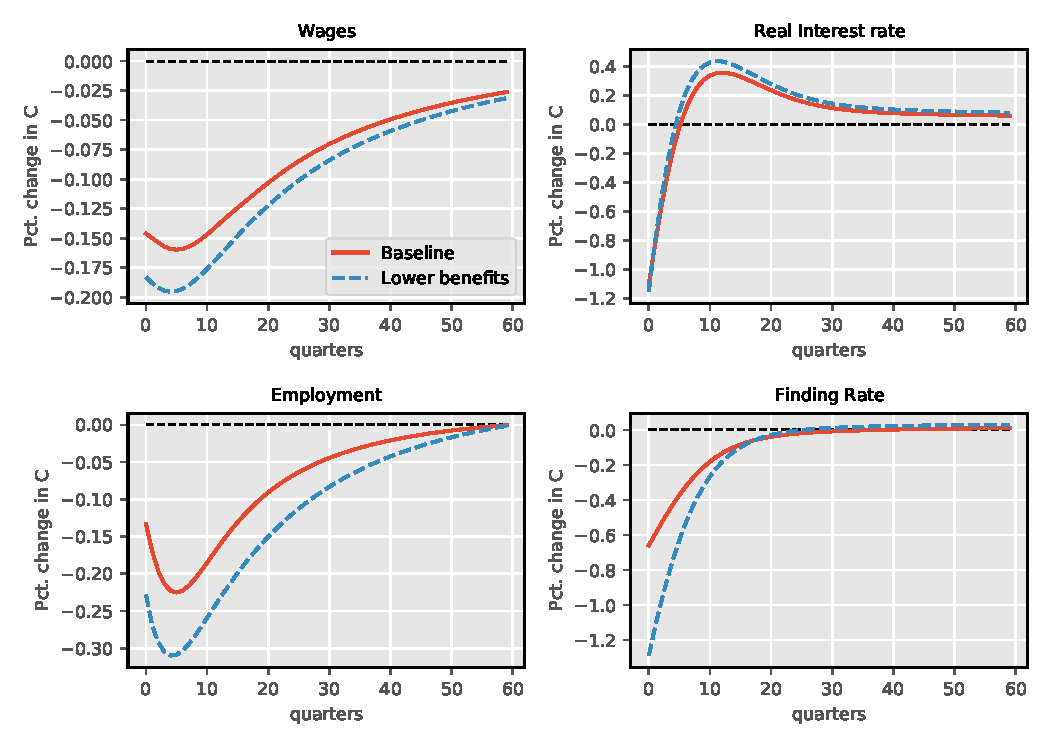
\includegraphics[width=.98\linewidth]{mainmatter/plots/Lower_b_main/main_result_C_decomp_G.pdf} 
}
\caption[Caption for LOF]{Consumption Decomposition.}
\label{fig:lower_b_C_decomp_G}
 % {\scriptsize  Impulse responses to a negative productivity shock of 1\% with persistence 0.94 (half-life: 5 quarters). }
\end{figure}




\subsubsection{Welfare Implications.}



\begin{figure}[H]
\makebox[\linewidth][c]{%
\centering
  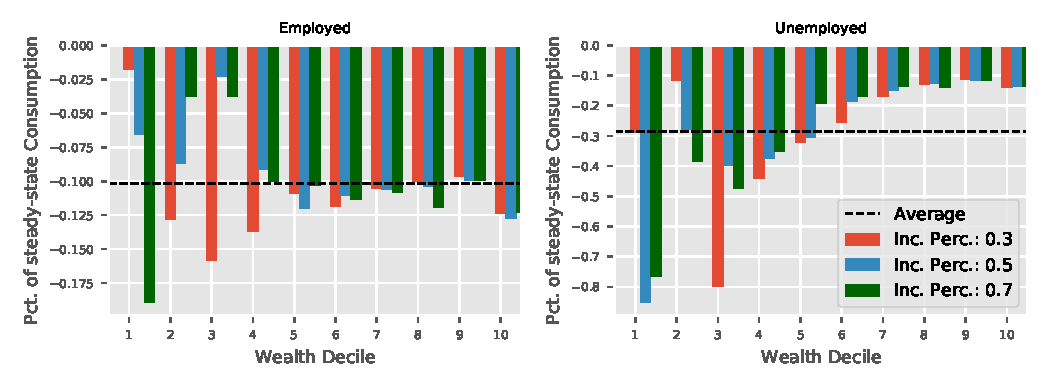
\includegraphics[width=.98\linewidth]{mainmatter/plots/Lower_b_main/equiv_welfare.pdf} 
}
\caption[Caption for LOF]{Consumption equivalent welfare losses from cutting unemployment benefits.}
\label{fig:lower_b_C_decomp_G}
 % {\scriptsize  Impulse responses to a negative productivity shock of 1\% with persistence 0.94 (half-life: 5 quarters). }
\end{figure}

\subsubsection{Aggregate Inequality.} Figure \ref{fig:Inequality_response_lower_b} in the appendix compares the changes in aggregate inequality. With lower unemployment insurance poor households save more for precautionary reasons and w
Consumption inequality increases as poor households cut consumption for precautionary reasons, but the aggregate effects are still neglectable.  





\subsection{Tax Financing}
The presence of heterogeneous households imply Ricardian equivalence does not hold in this model, and financing government activities with taxes versus bonds alter the dynamic responses of shocks. Though I consider the scenario where the government fiances its expenses by primarily issuing bonds as the baseline scenario, I here consider the alternative. At each instant in time the government adjusts lump-sum transfers, to be distributed uniformly across households, to satisfy their government constraint. This is standard in simpler NK models. 
Figure \ref{fig:lower_b_shocks_T} presents the general equilibrium outcomes. There is slight propagation in the first period for output, consumption, employment and job-finding rates, though the overall impulses are roughly unchanged under a lower benefit level. 
The decomposition in Figure \ref{fig:lower_b_C_decomp_T} shows that compared to the bonds-financing scenario, wages and transfers now determine the majority of the consumption response, with the effect of interest rate on consumption being roughly halved. Regarding the effects of unemployment benefits the conclusions are almost unchanged: A more volatile job-finding rate propagates the initial consumption decline, while a slightly more persistent employment slump generates a more persistent drop in consumption. The effects of wages, transfers and interest rates on consumption are the same.  


\begin{figure}[H]
\makebox[\linewidth][c]{%
\centering
  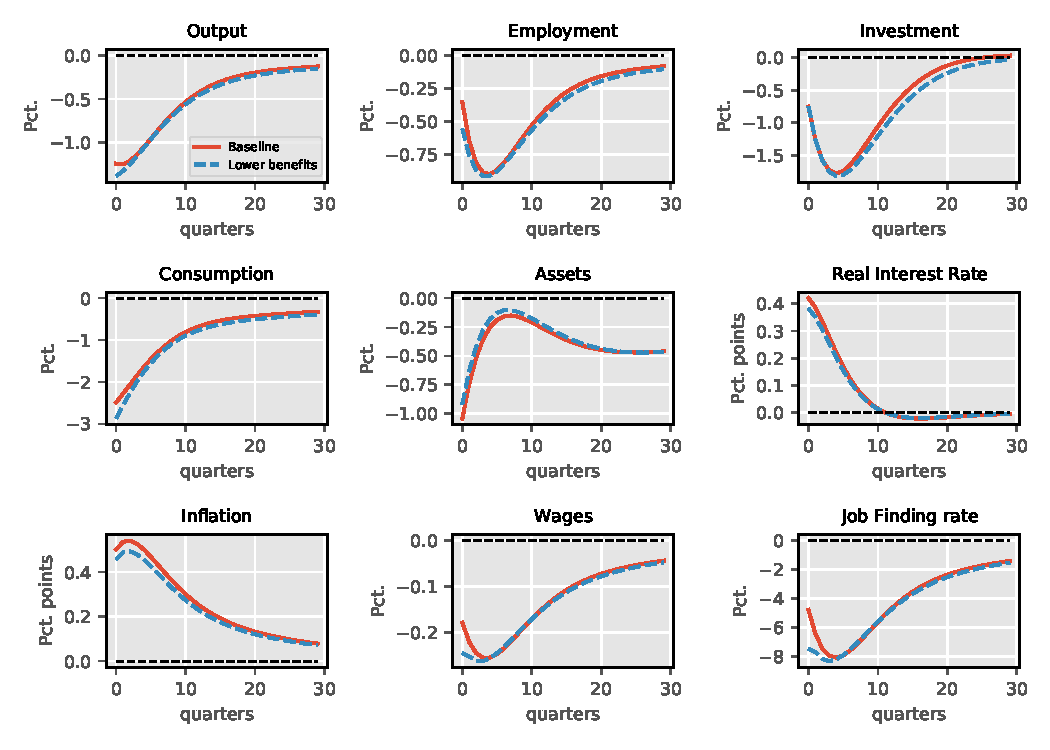
\includegraphics[width=.8\linewidth]{mainmatter/plots/Lower_b_main/main_result_comparison_T.pdf} 
}
\caption[Caption for LOF]{Consumption Decomposition.}
\label{fig:lower_b_shocks_T}
 % {\scriptsize  Impulse responses to a negative productivity shock of 1\% with persistence 0.94 (half-life: 5 quarters). }
\end{figure}


\begin{figure}[H]
\makebox[\linewidth][c]{%
\centering
  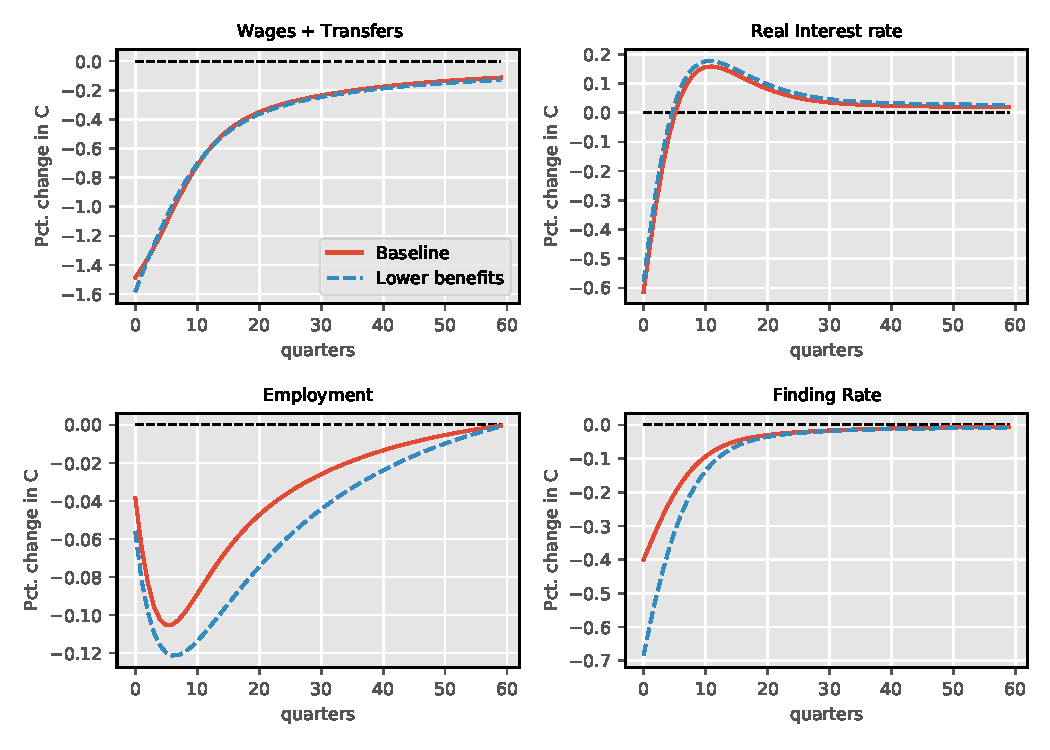
\includegraphics[width=.8\linewidth]{mainmatter/plots/Lower_b_main/main_result_C_decomp_T.pdf} 
}
\caption[Caption for LOF]{Consumption Decomposition.}
\label{fig:lower_b_C_decomp_T}
 % {\scriptsize  Impulse responses to a negative productivity shock of 1\% with persistence 0.94 (half-life: 5 quarters). }
\end{figure}


